\documentclass{llncs}
\usepackage[style=alphabetic,backend=bibtex]{biblatex}
\usepackage{graphicx}



\addbibresource{kwarc.bib}

\title{Demo: TGView3D for Immersive Theory Graph Exploration}
\author{Richard Marcus, Michael Kohlhase, Florian Rabe}
\institute{Computer Science, FAU Erlangen-N\"urnberg}

\begin{document}
\maketitle

It is difficult to represent mathematical knowledge efficiently due to its inherent complexity.
Modular representation formats like OMDoc/MMT~\cite{Kohlhase:OMDoc1.2,RabKoh:WSMSML13} organize it into theories with truth-preserving inclusions and interpretations (morphisms).
To help users understand the global and local structure of such representations and libaries, we have experimented with visualizing the theory graphs in the TGView~\cite{RupKohMue:fitgv17} system. But the sheer size of theory graphs -- they can contain thousands of nodes and an order of magnitude more edges -- complicates the use if no other processing is done before.

To cope with this, we propose an interactive virtual reality theory-graph viewer: TGView3D. This system follows TGView, which relies on two-dimensional representations. TGView already allows switching between several layouts such as a hierarchical or a force-directed one. Furthermore, nodes can be moved manually and different visual highlighting options are available.

Adding the depth as a third dimension to this concept helps to further organize the theory graph, as effectively more space is generated. Additionally, this offers an direct way of filtering the information. Since it is possible to freely navigate through the 3D-graph, the user can easily focus on the current visible slice.

Porting the system to virtual reality is the logical consequence. The first advantage is the extremely wide field of view. In combination with the head tracking, this allows for a natural exploration of the represented knowledge. Secondly, special controllers simulate functions of the human hand, e.g. grabbing and pointing, which offers intuitive ways of interaction in the three-dimensional world. Last, the immersive experience of virtual reality results in stronger stimulation of brain areas involved in spatial cognition compared to traditional computer graphics. This could possibly help finding certain patterns in the graph.



\begin{figure}
    \centering
    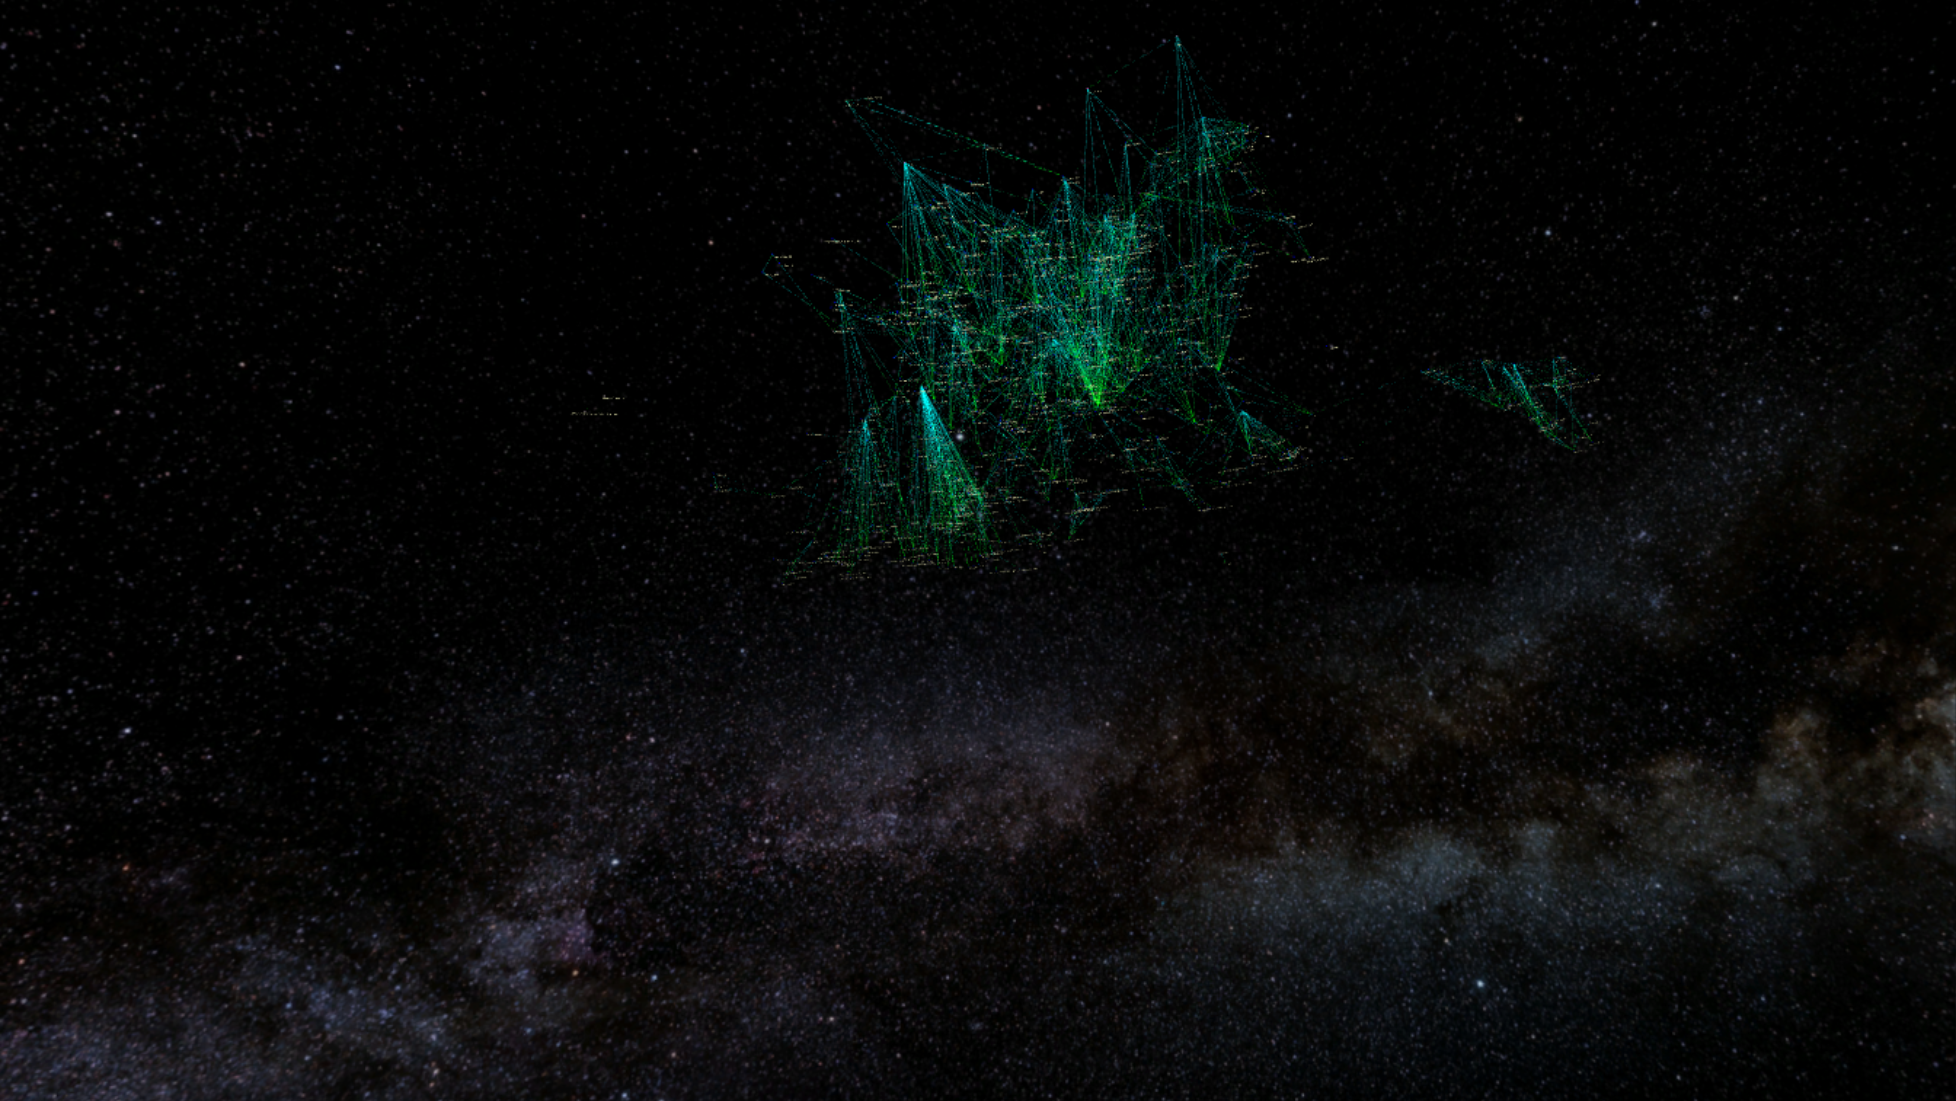
\includegraphics[width=1\textwidth ]{galaxyfaraway}
    \caption{The graph is positioned in the 3D space. Possibly, further graphs can be placed in relation to each other.}
    \label{fig:sample_figure1}
\end{figure}

\begin{figure}
    \centering
    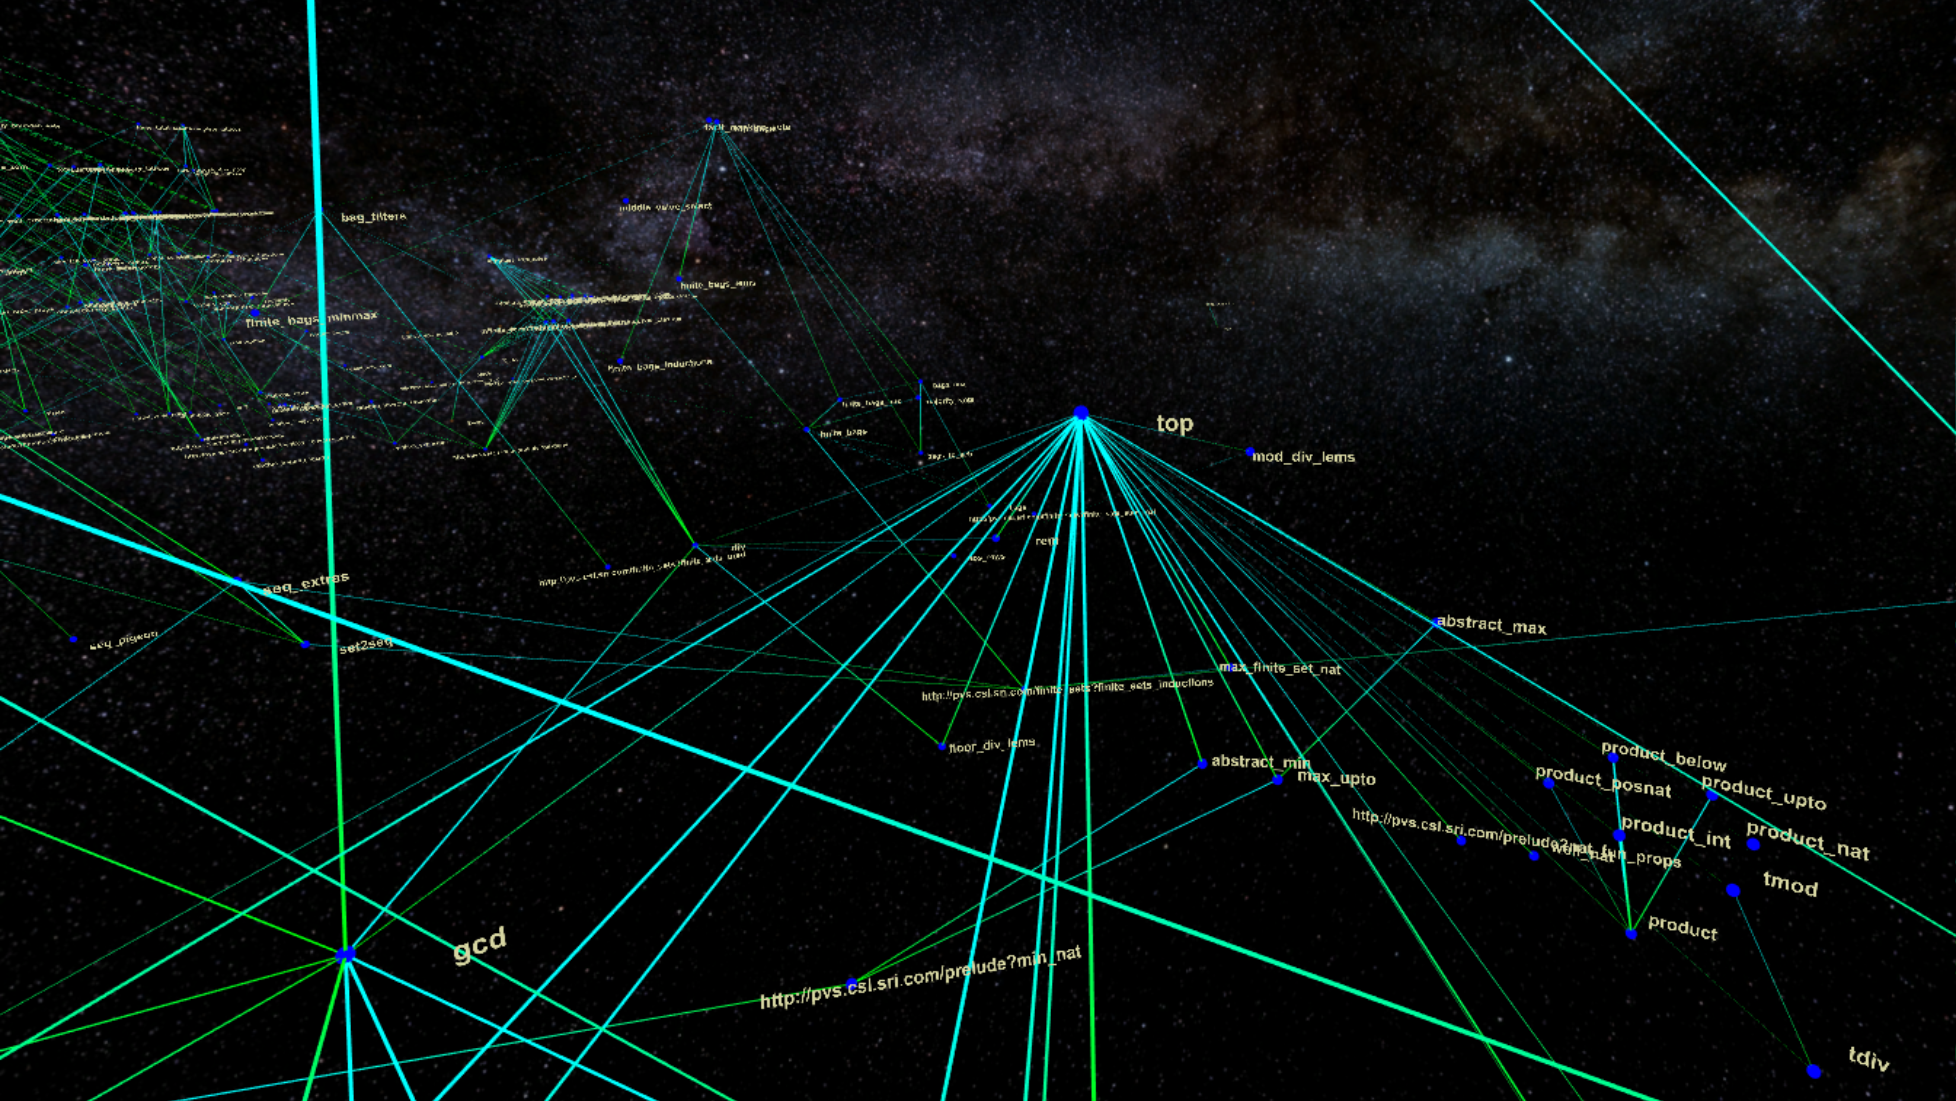
\includegraphics[width=1\textwidth ]{part}
    \caption{The user can move through the world freely. This allows inspecting parts of the graph in detail. The edges have color gradients according to their directions.}
    \label{fig:sample_figure2}
\end{figure}


\begin{figure}
    \centering
    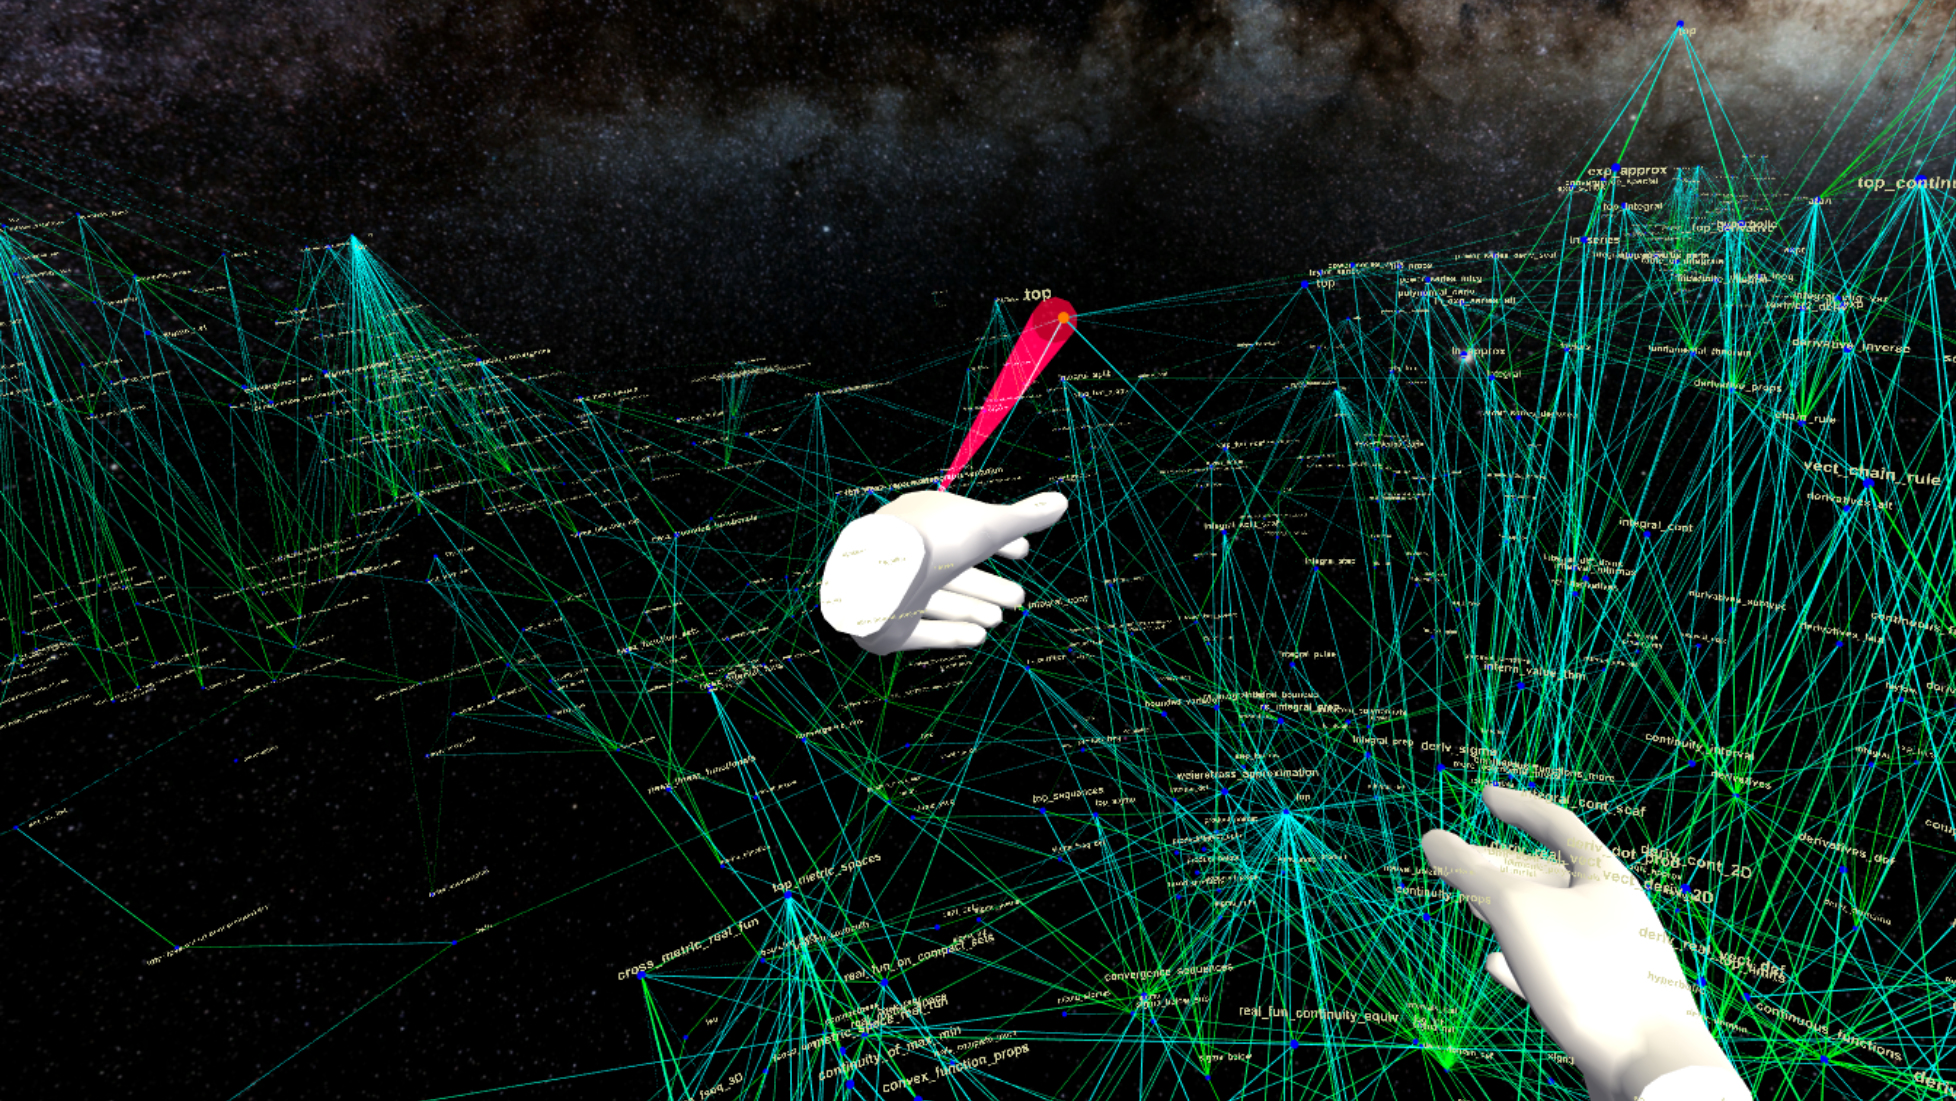
\includegraphics[width=1\textwidth ]{tractor}
    \caption{Nodes can be dragged towards the user with the help of a tractor beam.}
    \label{fig:sample_figure3}
\end{figure}

\begin{figure}\centering
    \includegraphics[width=1\textwidth ]{grab}
    \caption{If the nodes are close enough, they land in the hands of the user and can be dragged to another place}
    \label{fig:sample_figure4}
\end{figure}

In order to optimize the 3D-viewer, we will tailor current functionalities towards the
requirements of a virtual reality application, create specialized graph layout algorithms
and find smart ways of showing the relevant pieces of information. By doing this, we
hope to not only create a system that can present theory graphs in a structured and
intuitive way, but also aid mathematicians in discovering new theories.

The TGView3D system is written in the unity3D framework (\url{https://unity3d.com/}) and the code is available at \url{https://github.com/UniFormal/TGView3D} under the GPLv3 license.
The graph viewer is supposed to work on a regular monitor as well as on the Oculus Rift. Unity builds will be released, as soon as the prototypes are fully stable.

\printbibliography
\end{document}

 
%%% Local Variables:
%%% mode: latex
%%% mode: visual-line
%%% fill-column: 5000
%%% TeX-master: t
%%% End:
